% Author: Izaak Neutelings (March 2019)
\documentclass[border=3pt,tikz]{standalone}
\usepackage{ifthen}
\usepackage{siunitx}
\tikzset{>=latex} % for LaTeX arrow head


\begin{document}



% ENERGY LEVELS
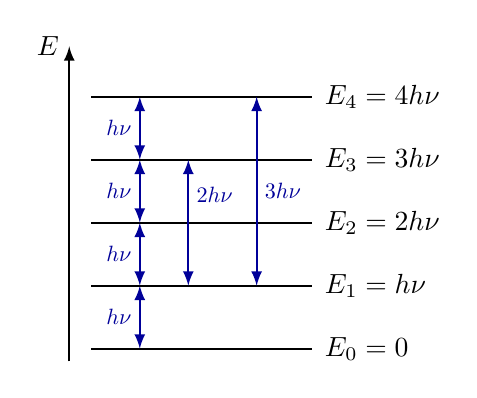
\begin{tikzpicture}[xscale=2.8,yscale=0.8]
  
  \foreach \n in {0,...,4}{
    \ifthenelse{\n>1}{
      \draw[thick] (0,\n) --++ (1,0) node[right=1pt] {$E_{\n}=\n h\nu$};
    }{\ifthenelse{\n>0}{
      \draw[thick] (0,\n) --++ (1,0) node[right=1pt] {$E_{\n}=h\nu$};
    }{
      \draw[thick] (0,\n) --++ (1,0) node[right=1pt] {$E_{\n}=0$};
    }}
    \ifthenelse{\n<4}{
      \draw[<->,thick,blue!60!black] (0.22,\n) --++ (0,1) node[left,midway,scale=0.8] {$h\nu$};
    }
  }
  
  \draw[->,thick] (-0.1,-0.2) --++ (0,5) node[left] {$E$};
  
  \draw[<->,thick,blue!60!black] (0.44,1) --++ (0,2) node[above=10pt,right,midway,scale=0.8] {$2h\nu$};
  \draw[<->,thick,blue!60!black] (0.75,1) --++ (0,3) node[right,midway,scale=0.8] {$3h\nu$};
  
\end{tikzpicture}



\end{document}
